% ===================================================
% CHAPITRE 27 — AVENAS ET SON ÉGLISE
% Pages imprimées 276-281 — vues 279-284
% ===================================================
\chapter{Avenas et son église}

% --- Page imprimée 276 — vue 279
\begin{center}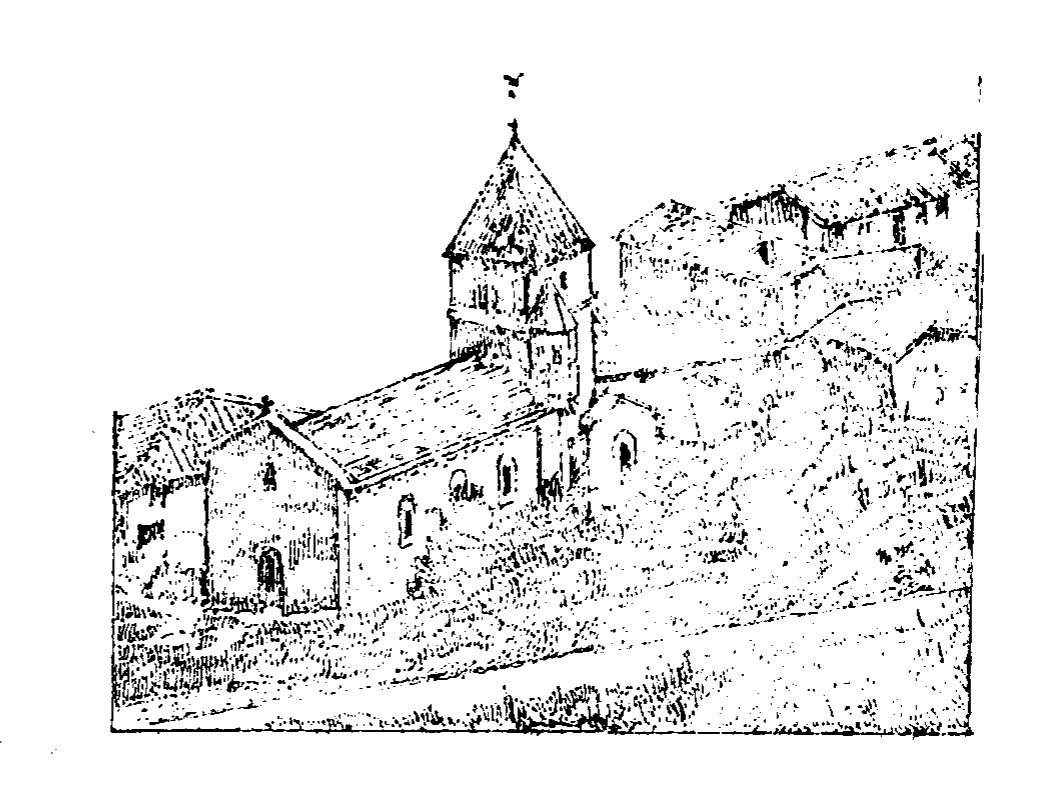
\includegraphics[width=0.62\textwidth]{Illustrations/illus-avenas-eglise.jpg}\end{center}

\ourouxlettrine{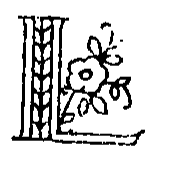
\includegraphics[height=4\baselineskip]{Illustrations/lettrines/lettrine-l.png}}{histoire de l'église d'Avenas n'entre pas dans le cadre de l'Histoire d'Ouroux. Cependant, dans l'histoire d'Ouroux, nous avons, à plusieurs reprises, parlé un peu des paroisses voisines. En ce qui concerne Avenas, nous avons mentionné plusieurs faits historiques qui se sont passés dans son château féodal.}

L'église d'Avenas abritant l'un des plus anciens autels de France et étant desservie par le curé résidant à Ouroux mérite, à ce double titre, une place et une mention spéciales dans l'histoire d'Ouroux.

À part une ou deux remarques, nous nous contenterons de relever au sujet de l'histoire de cette petite paroisse et de son église un article paru dans « l'ESSOR » (journal catholique du Diocèse de Lyon) du 10 février 1952, signé par le journaliste A. JOROND.

% --- Page imprimée 277 — vue 280
\begin{quote}
« Avenas n'est qu'un petit village de 200 âmes (1) perdu dans les monts du Beaujolais, à quelque 600 mètres d'altitude, cependant son passé est riche de souvenirs et de légendes.

Son église et surtout son maître-autel unique en France font l'admiration de l'archéologue, de l'historien et du touriste averti.

Au IXe siècle il existait déjà, au milieu de la forêt, une abbaye de religieuses suivant la règle de Saint-Benoît : le monastère de Pélage. Lors de leur repli vers l'Orient, les Sarrasins détruisirent cet édifice et égorgèrent les moniales.

Toutefois l'abbesse Anstrude échappa miraculeusement au massacre et mit l'avenir de la communauté sous la protection de Charlemagne. Le grand empereur, défenseur de la chrétienté, lui assura aide et protection et chassa les barbares.

La paroisse prit le nom d'Avenacum pour s'appeler plus tard « Avenus », puis « Avenas ».

Pourquoi ce nom ? On croit savoir que c'est en raison de la production principale de son territoire : l'avoine. La paroisse aurait en effet tiré son appellation du mot latin « avena ». Cette thèse est certes fort discutable. Ne serait-ce pas plutôt le nom de la princesse Avana, sœur de Guillaume le pieux, fondateur de Cluny, qui avait comblé de bienfaits la contrée ?

Quoi qu'il en soit, l'église d'Avenas fut érigée au 9ème siècle sur l'emplacement de l'antique monastère du Pélage.

Les curés d'Avenas furent, pendant plusieurs siècles, des moines bénédictins dépendant de l'abbaye de Cluny.

La légende de Ganelon.

Louis le Débonnaire, dit Louis le Pieux, fils de Charlemagne, traversa, dit-on, Avenas en 814, à la poursuite du traître Ganelon, cause de la mort de Roland à Roncevaux. Ganelon possédait un puissant château au sommet du Fourvéon. Seigneur du lieu, il exerçait un pouvoir tyrannique sur ses malheureux sujets. Louis le Débonnaire l'attaqua dans sa forteresse dont il fit raser les tours. Le traître s'étant enfui fut rattrapé par ceux qu'il avait persécutés.

\end{quote}
------------

Note. Avenas comptait au dernier recensement 134 habitants.

% --- Page imprimée 278 — vue 281
\begin{center}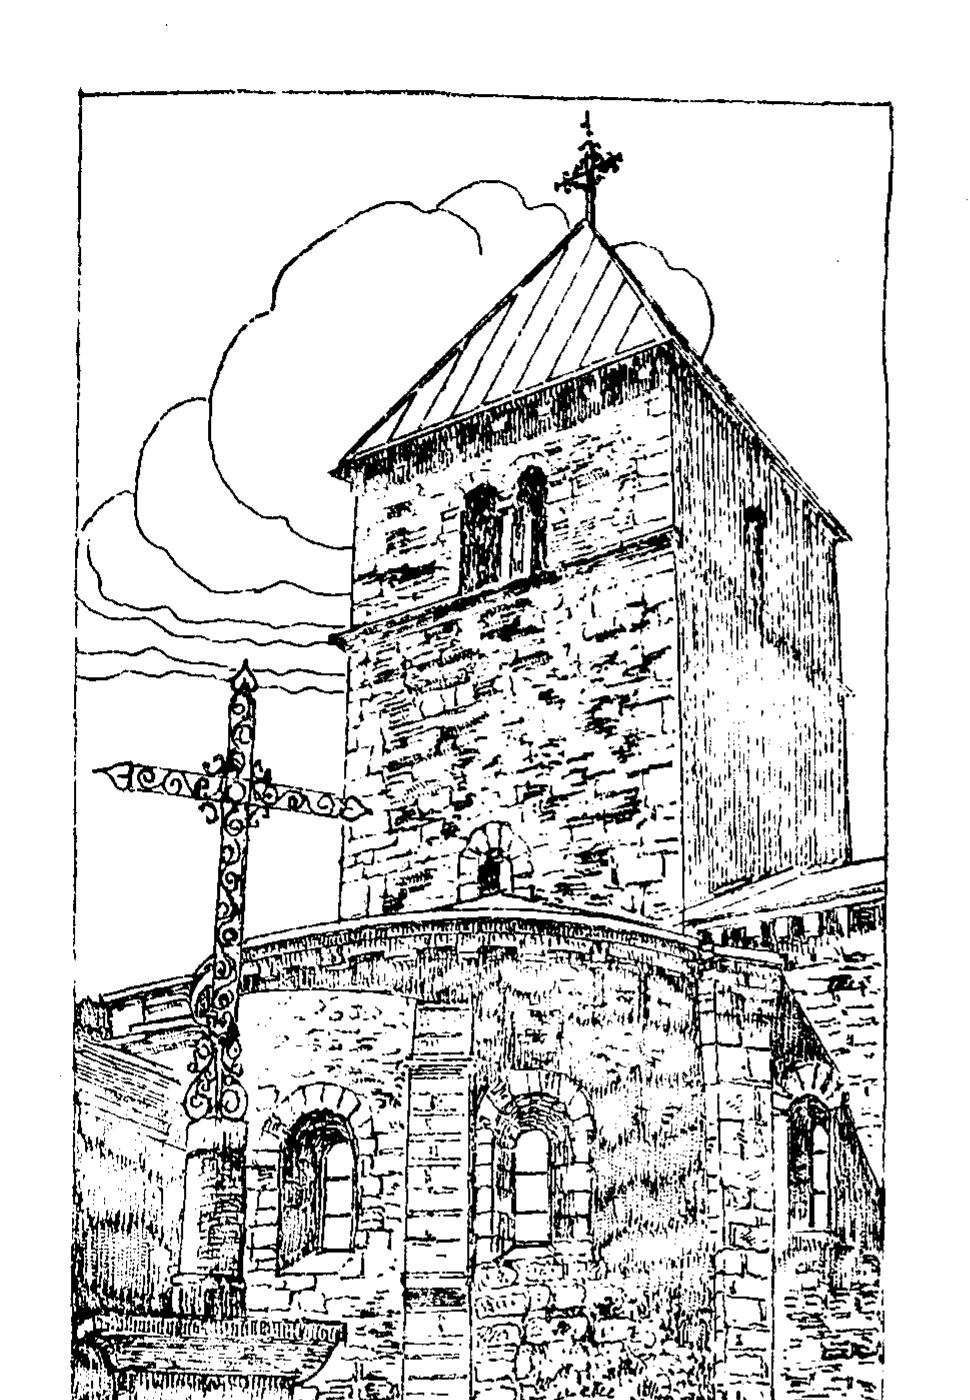
\includegraphics[width=0.62\textwidth]{Illustrations/illus-avenas-croix.jpg}\end{center}

L'église d'Avenas et la nouvelle croix, bénite le 4 juin de l'année 1950.

Cette croix, en fer forgé, est l'œuvre de Mr Laurent Callot, maréchal-ferrant d'Avenas. Pour réaliser ce travail il s'est inspiré de plusieurs dessins dus à la main de Mr Mondon du château de Quillin.

L'église d'Avenas a été restaurée en 1906 par l'architecte lyonnais LENAIL. Comme style elle appartient au roman de transition où l'ogive commence à apparaître.

La tradition rapporte que Ganelon fut enfermé dans un tonneau garni de pointes à l'intérieur. Le fût ayant été hissé à la cime du Fourvéon, on lui fit dévaler la pente de la montagne.

Telle est la légende que l'on raconte encore à Chénellette. Quel crédit faut-il y attacher ?

Certains auteurs estiment que ce personnage est purement imaginaire ; d'autres, au contraire, prétendent qu'il fut tué à Laon, en 788.

Le cartulaire de Saint-Vincent de Mâcon, qui relate les origines du diocèse de Mâcon, semble nous faire admettre cette première version. Ce serait en commémoration de sa victoire sur le traître que Louis le Pieux aurait fait ériger l'église paroissiale d'Avenas.

\ourouxsubtitle{L'autel carolingien d'Avenas}

L'autel monumental de l'église d'Avenas est un trésor artistique d'une inestimable valeur. Rares sont les monuments remontant à une époque aussi reculée, mis à part Germigny-les-Prés, dans le Loiret, qui possède une chapelle et des fonts baptismaux datant de Charlemagne.

% --- Page imprimée 279 — vue 282
Le Beaujolais peut être fier de posséder l'autel d'Avenas, qui est, à n'en pas douter, du plus pur style carolingien. Sculptures primitives, rustiques, très provinciales, mais combien édifiantes.

Cette pièce d'art, en calcaire blanc, aurait été exécutée à Beaujeu par des artistes du terroir peu de temps après la mort de Louis le Pieux, en 840, puisque l'on peut y lire le jour et le mois de la mort du roi.

Les scènes représentées dans les trois bas-reliefs de l'œuvre sont extrêmement curieuses. Conception naïve peut-être, mais bien significative.

Sur la face antérieure de l'autel, on peut voir le Christ assis sur un trône dans un médaillon de forme elliptique ogivique. Il faut regretter que les mutilations aient déformé le sujet. Sur deux rangs superposés sont représentés les douze disciples de Jésus. L'ensemble symbolise la mission des apôtres dans le monde : « Qui crediderit et baptizatus fuerit salvus erit ».

Du côté de l'Épître, les sculptures de l'époque ont voulu reproduire le geste de Louis le Pieux offrant l'église d'Avenas telle qu'on peut la voir aujourd'hui.

« Rex Ludovicus pius et virtutes amicus. Offert ecclesiam. Recepit Vincentius istam. Lampada bissena fluxurus Julius ibat. Mors fugat obpositum Regis ab interitum ».

« Le roi Louis le Pieux, ami de la vertu, offre cette église. Vincent la reçoit. Après douze soleils, juillet allait commencer son cours. La mort écarte les gages présentés pour conjurer le décès du roi. »

Ce texte concorde avec celui du cartulaire de Saint-Vincent de Mâcon en 815 de l'église d'Avenas par Louis le Débonnaire.

Les sujets du troisième bas-relief sont plus difficiles à interpréter. M. le chanoine Cucherat, auteur d'une étude historique sur Avenas, nous donne cette explication : le personnage représenté sur son lit de mort n'est autre que Louis le Pieux, à qui la Vierge et l'enfant Jésus apparaissent en récompense de sa foi inébranlable et de ses bonnes œuvres. Le compartiment supérieur représente l'Annonciation et la Présentation au Temple.

% --- Page imprimée 280 — vue 283
M. le chanoine Cucherat est formel sur ce point. Il apparaît donc vraisemblable que l'autel et ses inscriptions se rapportent bien au fils de Charlemagne et non à saint Louis, comme certains historiens l'ont prétendu. (Voir notes à la page suivante.)

Ce qui a pu induire ceux-ci dans l'erreur, c'est qu'en effet, le roi-chevalier se rendant aux croisades suivit la voie romaine qui traverse le village, en 1248 et dont on retrouve encore des vestiges.

L'église d'Avenas est aussi du plus pur style roman, cependant des restaurations récentes ont modifié légèrement son aspect primitif. »

Note. Dans le bas-relief du côté de l'Évangile beaucoup ne sont pas de l'avis du chanoine Cucherat et voient là quatre scènes se rapportant à la vie de la Sainte Vierge : 1° à gauche, en bas c'est la naissance de la Sainte Vierge. Une femme est allaitée (Ste Anne), une autre femme, debout (sage-femme) tenant un enfant nouveau-né (Marie) ; 2° en haut à gauche c'est l'Annonciation ; 3° en haut, à droite c'est la Présentation ; 4° en bas, à droite c'est l'Assomption de la Ste Vierge. La femme allaitée c'est la Ste Vierge avec St-Jean à ses pieds et St-Pierre à son chevet qui pleurent. Un buste enlevé dans un voile c'est la montée au ciel de Marie.

Sur la face antérieure de l'autel, le Christ est assis dans un médaillon en creux ; à droite et à gauche, sur deux rangs superposés, 3 à 3 les 12 apôtres, le livre des évangiles à la main à l'exception de Judas qui a les mains vides.

\begin{center}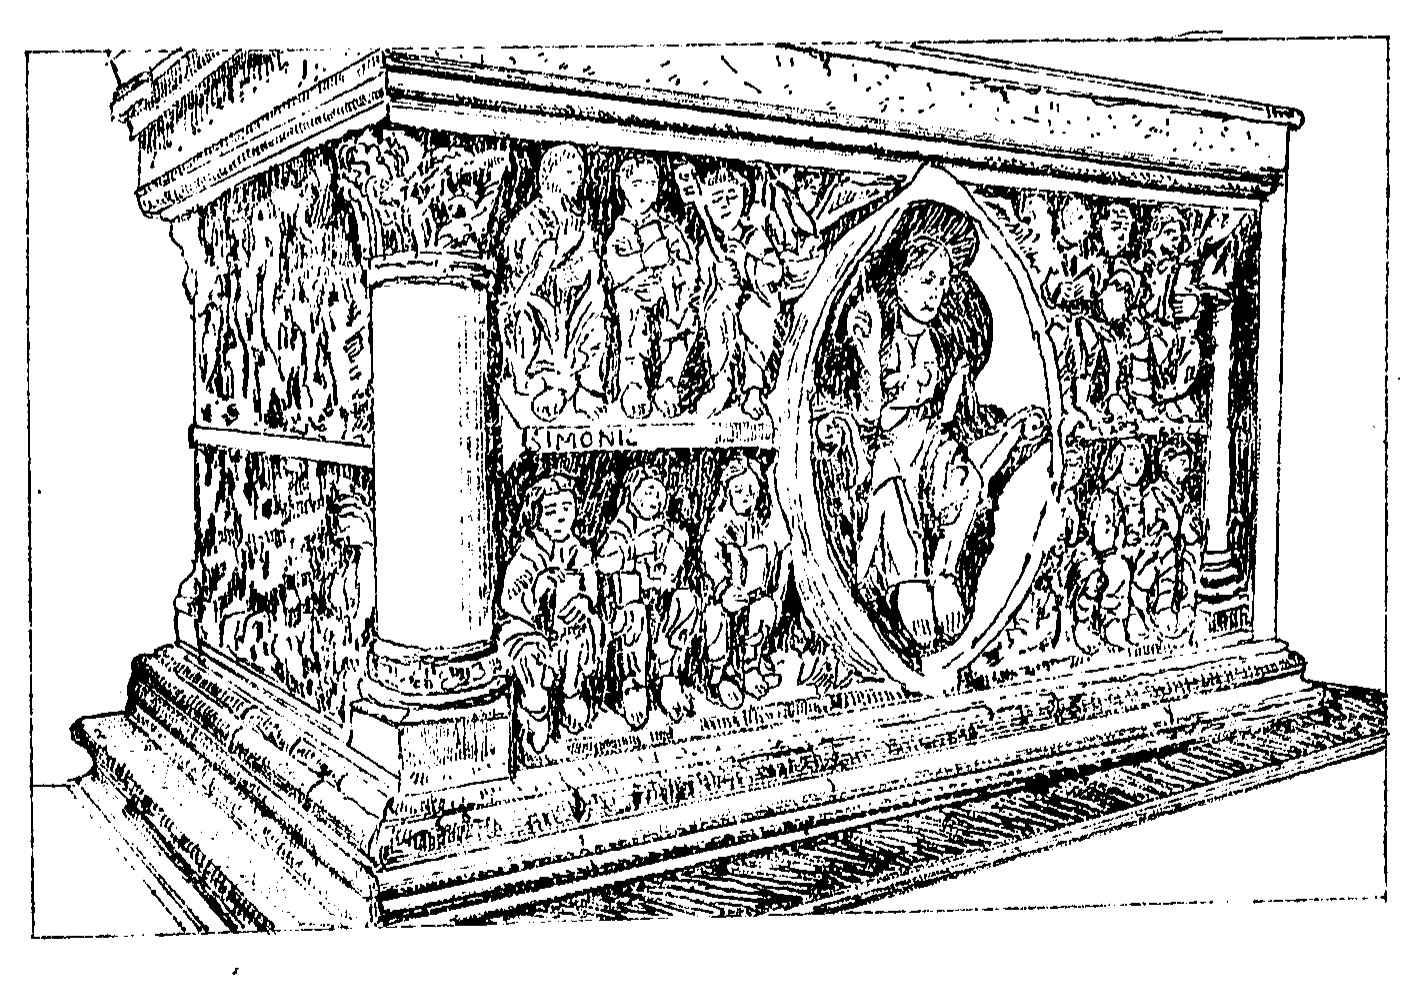
\includegraphics[width=0.62\textwidth]{Illustrations/illus-autel-avenas-bas-relief.jpg}\end{center}

% --- Page imprimée 281 — vue 284
Note à propos de la date de l'autel d'Avenas

Il y a à ce sujet plusieurs opinions, mais deux principales sont à signaler. Nous vous les donnons telles que Mr Mondon du château d'Avenas les a résumées.

1ère opinion : SEVERT, chanoine de Beaujeu est le premier qui ait fait connaître cet autel. Il lui fut signalé par Mgr LIMET, évêque de Mâcon qui l'avait découvert pendant le cours d'une visite paroissiale. Notre historien nous dit que Louis le Débonnaire se rendant à Aix-en-Provence en 824 ou 830 pour assister à un concile, passa par Avenas où il s'arrêta chez des religieux qui avaient un couvent situé vraisemblablement au « Bât d'Avenas ». Il profita de son séjour en ce lieu pour faire démolir le château de Fourvéon, ancienne retraite du traître Ganelon que Charlemagne avait vaincu. En commémoration de cette victoire, Louis le Débonnaire aurait fait édifier l'église et l'autel d'Avenas. Mais, ajoute Severt, tout cela n'est fondé que sur une commune tradition.

2ème opinion : C'est celle de Mr Ferdinand de la Roche de la Carelle. Ne reconnaissant pas dans l'autel d'Avenas les caractères de l'architecture carolingienne, il refuse de lui donner une date aussi reculée sans relater toutes les preuves secondaires qu'il apporte pour appuyer sa thèse, venons au principal motif qui le détermine à attribuer l'autel d'Avenas à St-Louis, neuvième du nom et roi de France. Il affirme que les qualificatifs PIUS et VIRTUTIS AMICUS semblent convenir merveilleusement au roi que l'Église a décoré de l'auréole des saints.

Pour corroborer son opinion, il cherche à démontrer que saint Louis passa à Avenas, quand, partant pour la croisade il alla s'embarquer à Aiguesmortes le 25 août 1248. Reste à trouver le véritable motif de l'érection indiqué par le dernier vers de l'inscription :

MORS FUGAT OBPOSITV REGIS AD INTITUM

Il le trouve dans la cessation spontanée d'une de ces épidémies si fréquentes au moyen-âge et qu'il attribue à l'intervention du saint roi. « La mort fuit à l'aspect du Roi ».

Pour conclure, chacun restant libre de choisir la thèse qui lui paraît la plus vraisemblable, nous disons « ad libitum ».

\enlargethispage{2\baselineskip}
\begin{center}
\vspace{-0.5\baselineskip}
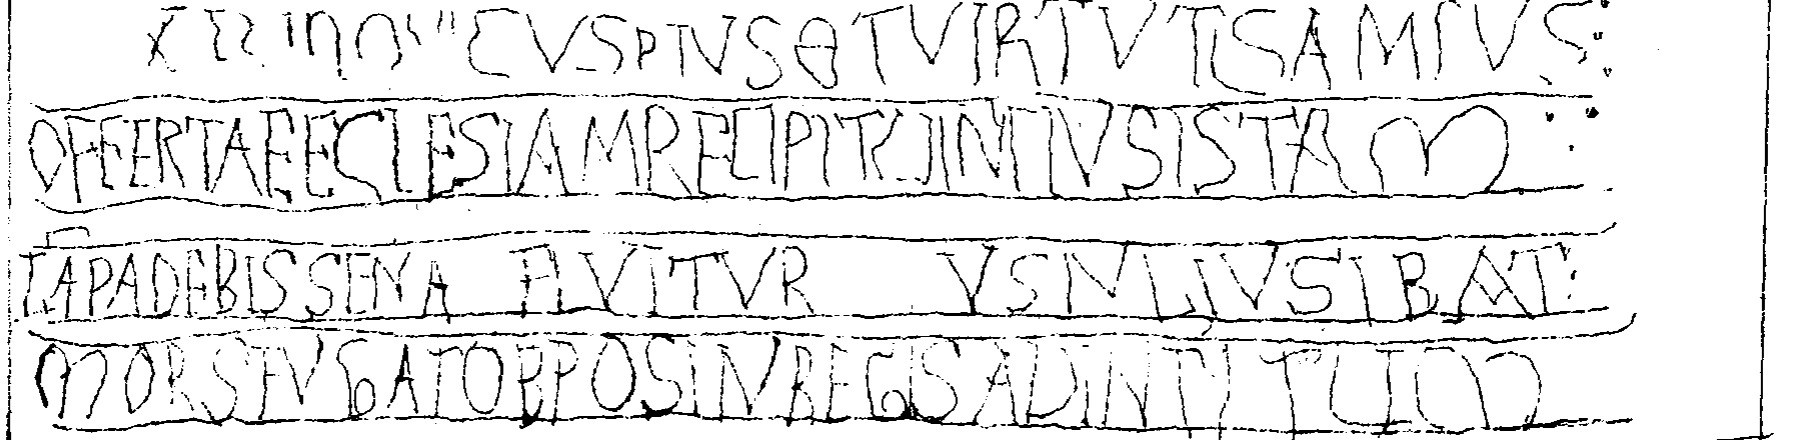
\includegraphics[width=0.52\textwidth]{Illustrations/illus-autel-avenas-inscription.jpg}
\end{center}

(RE)X LVDOVICVS PIVS ET VIRTVTIS AMICVS  
OFFERT ECCLESIAM RECEPIT VINCENTIVS ISTAM  
LAMPADA BISSENA FLVITVRVS IVLIVS IBAT  
MORS FVGAT OBPOSITV REGIS AD INTITVM

(Inscription de l'autel d'Avenas, côté de l'Épître)
